\begin{frame}{Model Description: Plackett-Luce observation model}

Model 1 (without seniority covariates)
    \begin{itemize}
        \item skills: $\lambda_i\in\mathbb{R}$ for player $i\in 1, \dots, n$
        \item $m$ participated players: $\left\{i_{1}, \ldots, i_{m}\right\} \subset \{1,2, \ldots, n\}$ for some $1\le m\le n$
        \item random rank outcome $O$: random vector $O = (O_1, \dots, O_m)$ takes values in $\mathcal{P}_{i_{1}, \ldots, i_{m}}$, the permutation set of $\left\{i_{1}, \ldots, i_{m}\right\}$
        \item likelihood: for any possible outcome $o = (o_1, \dots, o_m)\in \mathcal{P}_{i_{1}, \ldots, i_{m}}$,
        \begin{equation*}
        \operatorname{Pr}\{O=o \mid \lambda\}=\prod_{i=1}^{m} \frac{\exp \left(\lambda_{o_{i}}\right)}{\sum_{j=i}^{m} \exp \left(\lambda_{o_{j}}\right)}
        \end{equation*}
    \end{itemize}
\end{frame}

\begin{frame}{Model Description: Plackett-Luce observation model}

Model 2 (with seniority covariates)
    \begin{itemize}
        \item seniority: $\beta_i \in\mathbb{R}$ for player $i\in 1, \dots, n$
        \item skills: $\lambda_i\in\mathbb{R}$ for player $i\in 1, \dots, n$
        \item $m$ participated players: $\left\{i_{1}, \ldots, i_{m}\right\} \subset \{1,2, \ldots, n\}$ for some $1\le m\le n$
        \item random rank outcome $O$: random vector $O = (O_1, \dots, O_m)$ takes values in $\mathcal{P}_{i_{1}, \ldots, i_{m}}$, the permutation set of $\left\{i_{1}, \ldots, i_{m}\right\}$
        \item likelihood: for any possible outcome $o = (o_1, \dots, o_m)\in \mathcal{P}_{i_{1}, \ldots, i_{m}}$,
        \begin{equation*}
        \operatorname{Pr}\{O=o \mid \lambda\}=\prod_{i=1}^{m} \frac{\exp \left(\lambda_{o_{i}} + \beta_{e_i}\right)}{\sum_{j=i}^{m} \exp \left(\lambda_{o_{j}} + \beta_{e_j}\right)}
        \end{equation*}
        $e_i$ is the seniority rank of player $o_i$
    \end{itemize}
\end{frame}

\begin{frame}{Specifying Priors on $\lambda$ and $\beta$}
    We want the prior to have good properties
    \begin{itemize}
        \item non-informative with respect to the relative skills of the players and the advantage for seniority
        \item all permutations $o \in \mathcal{P}_{i_1, \dots, i_m}$ are equally probable
        \item the priors of $\lambda_i, \beta_i$ for each player $i$ defined on $\mathbb{R}$
    \end{itemize}
    choose $\lambda_i, \beta_i \stackrel{\text{i.i.d}}{\sim}\text{certain $t$ distribution}$
\end{frame}

\begin{frame}{Checking the Priors}
Simulation results suggest choosing the prior $t_5$.

Setup:
\begin{itemize}
    \item focus on players 1, 2, 3
    \item simulate $10,000$ samples from the priors $\lambda_{o_{i}} \stackrel{\text{i.i.d}}{\sim} t_5$
    \item for each random permutation $o \in \mathcal{P}_{1, 2, 3}$, plot the density of $\operatorname{Pr}\{O=o \mid \lambda\}$
\end{itemize}
\end{frame}

\begin{frame}{Checking the Priors}

\begin{figure}
  \centering
  \begin{tabular}[b]{c}
    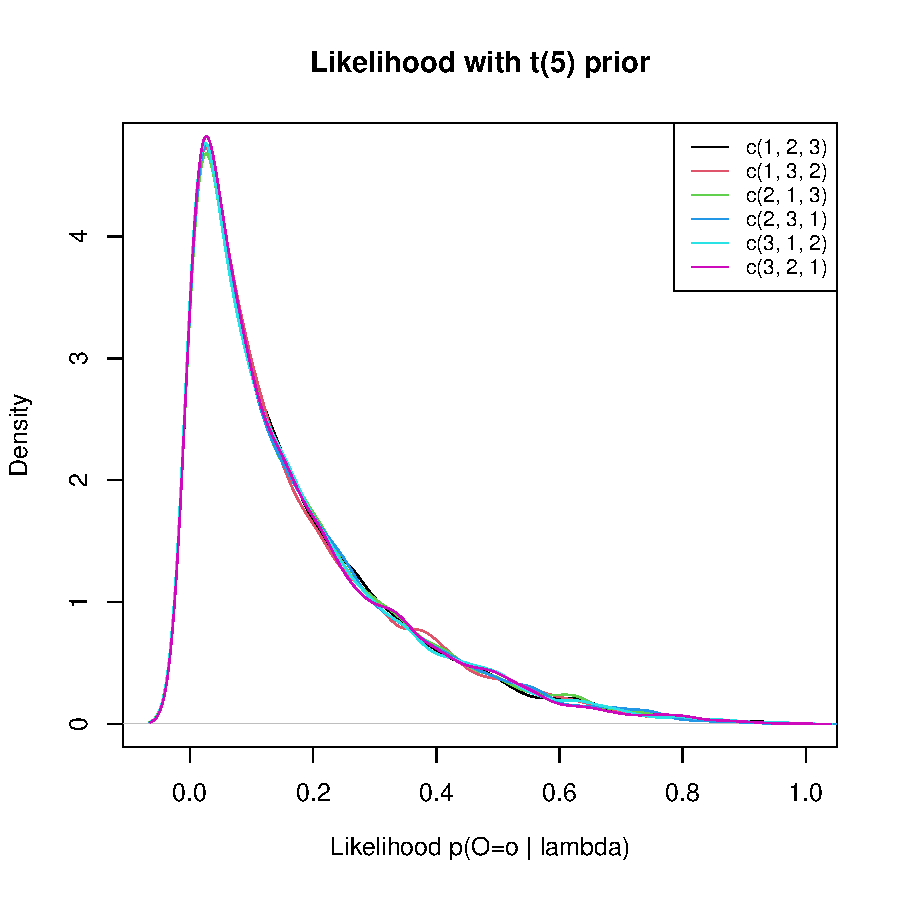
\includegraphics[width=.4\linewidth]{img/one_t5.pdf} \\
    \small (a) $t_5$
  \end{tabular} \qquad
  \begin{tabular}[b]{c}
    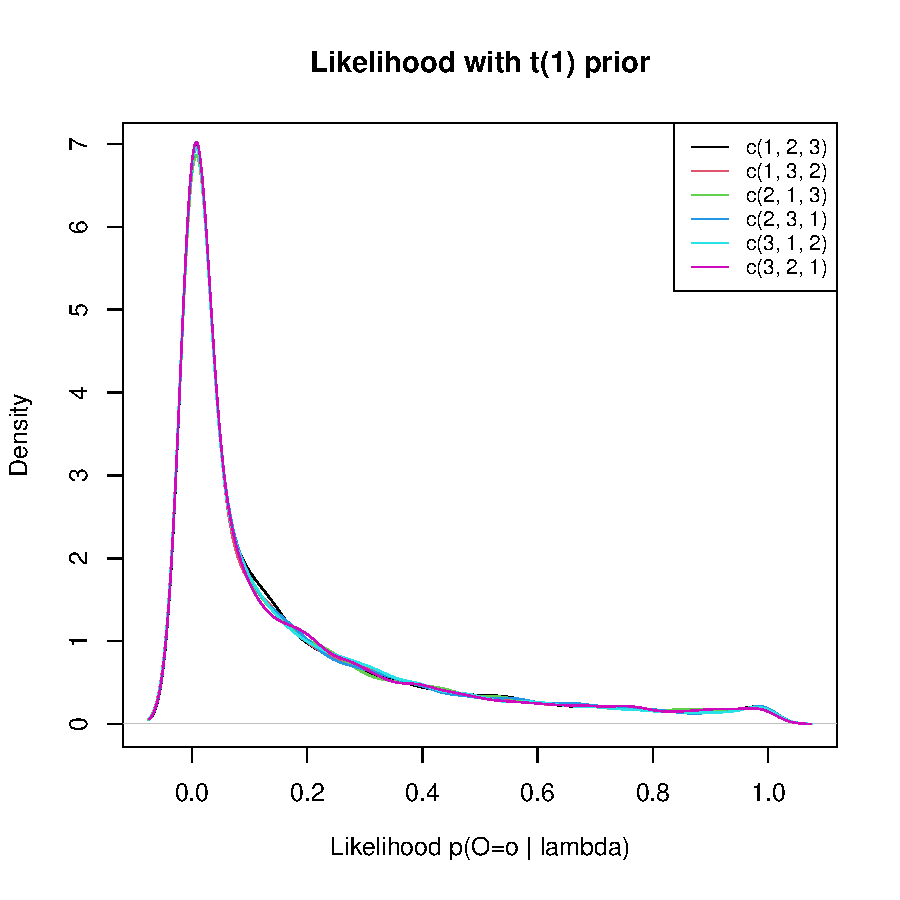
\includegraphics[width=.4\linewidth]{img/one_t1.pdf} \\
    \small (b) $t_1$
  \end{tabular}
  \caption{Comparison of $t_5$ prior and $t_1$ prior in model 1. }
\end{figure}
\vspace{-1em}
\begin{itemize}
    \item all density curves coincide $\implies$ the prior is non-informative \& all permutations are equally probable
    \item $t_5$ less concentrated around zero than $t_1$ $\implies$ $t_5$ induces more randomness in the game, and hence more preferred
    \item similar observation for model 2
\end{itemize}
\end{frame}
